\section{Proof of the Main Theorems}
\label{section:differentiable}

The proofs of Theorems \ref{DifferentiableIsPspace} and \ref{KTimesIsCH}
proceed as follows. 
In Sect.~\ref{section:divp}, 
we define \emph{difference equations}, 
a discrete version of the differential equations. 
In Sect.~\ref{subsection: counting hierarchy}, 
we show the $\classPSPACE$- and $\classCH$-hardness of 
difference equations with certain restrictions. 
In Sect.~\ref{subsection: ode family}, 
we show that these classes of difference equations can be simulated
by families of differential equations 
satisfying certain uniform bounds on higher-order derivatives. 
In Sect.~\ref{subsection: proof of theorems}, 
we prove the theorems by
putting these families of functions together 
to obtain one differential equation 
having the desired smoothness 
($\classC ^{(\infty, 1)}$ and $\classC ^{(\infty, k)}$). 

The idea of simulating a discrete system of limited feedback capability
by differential equations
was essentially already present in the proof of 
the Lipschitz version \cite{kawamura2010lipschitz}. 
% As explained there, the main idea 
% was to simulate $\classPSPACE$ computation by a discrete system 
% whose feedback capability is limited
% so that it could be simulated by a trajectory of 
% a Lipschitz continuous differential equation. 
We look more closely at this limited feedback mechanism, 
and observe that this restriction is one on the \emph{height}
of the difference equation. 
We show that a stronger height restriction makes
the difference equation simulable by 
smoother differential equations, 
leading to the $\classCH$-hardness for $\classC ^{(\infty, k)}$ functions.

\subsection{Difference Equations}
\label{section:divp}

In this section, we define difference equations, 
a discrete version of differential equations,
and show the $\classPSPACE$- and $\classCH$-hardness of 
families of difference equations with different height restrictions. 

Let $[n]$ denote $\{0, \dots , n-1\}$.
Let $G \colon [P] \times [Q] \times [R] \to \{-1, 0, 1\}$ and
$H \colon [P + 1] \times [Q+1] \to [R]$. 
We say that $H$ is the solution of the \emph{difference equation} given by $G$
if for all $i \in [P]$ and $T \in [Q]$ (Fig.~\ref{fig:divp}), 
\begin{gather}
   H(i, 0) = H(0, T) = 0 \enspace , \label{eq:initial value}
\\
   H(i + 1, T + 1) - H(i+1, T) = G(i, T, H(i, T)) \enspace .  \label{eq:divp}
\end{gather}
We call $P$, $Q$ and $R$ the \emph{height}, \emph{width} and \emph{cell size} of
the difference equation.
The equations \eqref{eq:initial value} and \eqref{eq:divp} are similar to 
the initial condition $h(0) = 0$ and the equation $\D h(t) = g(t, h(t))$ 
in \eqref{eq:ode}, respectively.
In Sect.~\ref{subsection: ode family}, we will simulate difference equations by differential equations using this similarity.

\begin{figure}
 \begin{center}
  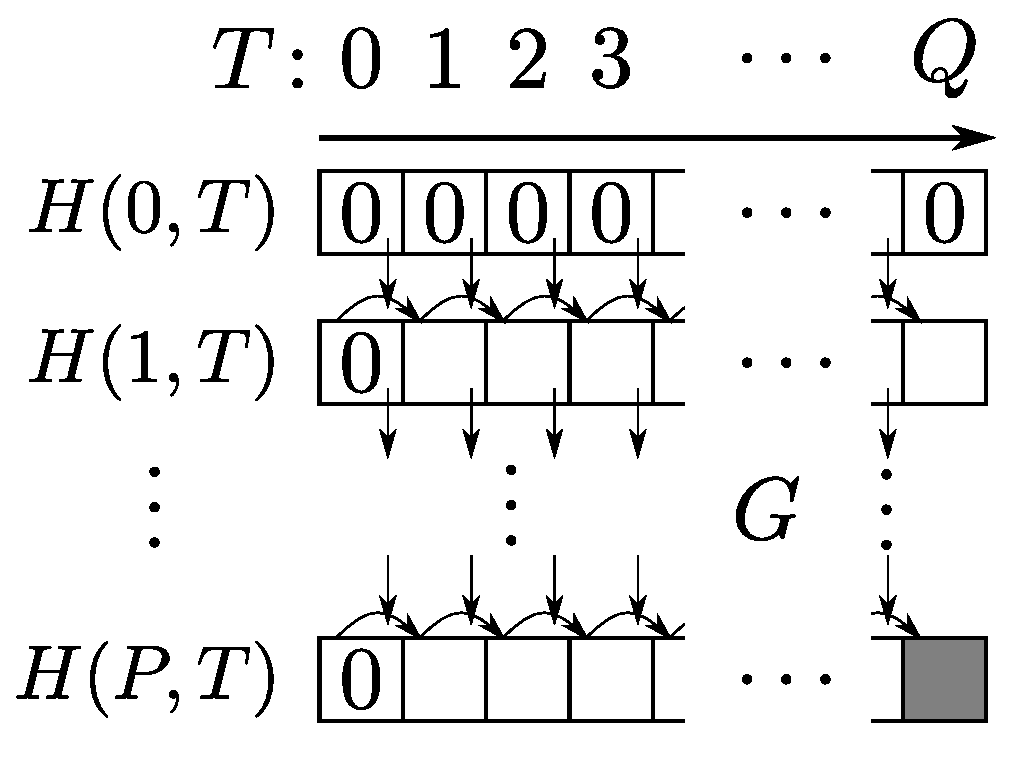
\includegraphics[height=0.15\textheight]{image/divp.eps}
 \end{center}
 \caption{The solution $H$ of the difference equation given by $G$}
 \label{fig:divp}
\end{figure}

We view a family of difference equations as a computing system by
regarding the value of the bottom right cell (the gray cell in Fig.~\ref{fig:divp}) as the output. 
A family $(G_u)_u$ of functions 
$G_u \colon [P_u] \times [Q_u] \times [R_u] \to \{-1, 0, 1\}$
\emph{recognizes} a language $L$ if for each $u$,
the difference equation given by $G_u$ has a solution $H_u$ 
and $H_u(P_u, Q_u) = L(u)$.
A family $(G_u)_u$ is \emph{uniform} 
if the height, width and cell size of $G_u$ are 
polynomial-time computable from $u$ (in particular, 
they must be bounded by $2^{p(|u|)}$, for some polynomial~$p$)
and $G_u(i, T, Y)$ is polynomial-time computable from $(u, i, T, Y)$.
A family $(G_u)_u$ has \emph{polynomial height} if the height $P_u$ is bounded by some polynomial $p(|u|)$.
A family $(G_u)_u$ has \emph{logarithmic height} if the height $P_u$ is bounded by $c \log |u| + d$ with some constants $c$ and $d$.
With this terminology,
the key lemma in 
\cite[Lemma 4.7]{kawamura2010lipschitz} 
can be written as follows:
\begin{lemma}
 \label{DIVPpolyIsPSPACEhard}
 There exists a $\classPSPACE$-hard language $L$ that is recognized by some uniform family of functions with polynomial height%
 \footnote{In fact, the languages recognized by 
 uniform families with polynomial height coincide with $\classPSPACE$.
}.
\end{lemma}

Kawamura obtained the hardness result in the third row in Table \ref{table:related} 
by simulating the difference equations of Lemma~\ref{DIVPpolyIsPSPACEhard}
by Lipschitz continuous differential equations. 
Likewise, 
Theorem~\ref{DifferentiableIsPspace} follows from Lemma~\ref{DIVPpolyIsPSPACEhard},
by a modified construction that keeps 
the function in class $\classC ^{(\infty, 1)}$ 
(Sects. \ref{subsection: ode family} and \ref{subsection: proof of theorems}).

We show further that 
difference equations restricted to have logarithmic height can be simulated by
$\classC ^{(\infty, k)}$ functions for each $k$ 
(Sects. \ref{subsection: ode family} and \ref{subsection: proof of theorems}).
Theorem~\ref{KTimesIsCH} follows from this simulation and the following lemma.
\begin{lemma}
 \label{DIVPlogIsCHhard}
 There exists a $\classCH$-hard language $L$ that is recognized by some uniform family of functions with logarithmic height.
\end{lemma}

The definition of the counting hierarchy $\classCH$, 
its connection to difference equations and 
the proof of Lemma~\ref{DIVPlogIsCHhard} 
will be presented in Sect.~\ref{subsection: counting hierarchy}. 



\subsection{The Counting Hierarchy and Difference Equations of Logarithmic Height}
\label{subsection: counting hierarchy}

The polynomial hierarchy~$\classPH$ is defined using non-deterministic polynomial-time oracle Turing machines: 
\begin{align}
 \classSigma^p_0  &= \classP \enspace ,
 &
 \classSigma^p_{n+1} &= \classNP ^{\classSigma^p_n} \enspace ,
 &
 \classPH &= \bigcup_n \classSigma^p_n \enspace .
\end{align}
The counting hierarchy~$\classCH$
is defined similarly
using probabilistic polynomial-time oracle Turing machines~%
\cite{wagner1986complexity,toran1991complexity}: 
\begin{align} \label{eq:CH}
 \quantC_0 \classP  &= \classP \enspace ,
 &
 \quantC_{n+1} \classP &= \classPP^{\quantC_n \classP} \enspace ,
 &
 \classCH &= \bigcup_n \quantC_n \classP \enspace .
\end{align}
It is known that $\classPH \subseteq \classCH \subseteq \classPSPACE$, 
but we do not know whether $\classPH = \classPSPACE$.


Each level of the counting hierarchy 
has a complete problem defined as follows.
For every formula $\phi(X)$ with the list $X$ of $l$ free propositional variables,
we write 
\begin{equation}
 \quantC^m X \phi(X) 
  \longleftrightarrow 
  \sum_{X \in \{0,1\}^l} \phi(X) \ge m \enspace ,
\end{equation}
where $\phi(X)$ is identified with the function 
$\phi \colon \{0,1\}^l \to \{0,1\}$
such that $\phi(X) = 1$ when $\phi(X)$ is true.
This ``counting quantifier'' $\quantC ^m$ generalizes 
the usual quantifiers $\exists$ and $\forall$, 
because $\quantC^1 = \exists$ and $\quantC^{2^l} = \forall$.
For lists $X _1$, \ldots, $X _n$ of variables 
and a formula $\phi(X_1, \dots, X_n)$ with all free variables listed, 
we define
\begin{equation}
 \langle \phi(X_1, \dots, X_n), m_1, \dots, m_n \rangle \in \quantC_n B_{\mathrm{be}}
 \longleftrightarrow
 \quantC^{m_n}{X_n} \cdots \quantC^{m_1}{X_1} \phi(X_1, \dots, X_n) \enspace .
\end{equation}

\begin{lemma}[{\cite[Theorem 7]{wagner1986complexity}}] \label{lemma:CnP-complete}
 For every $n \ge 1$, 
 the problem $\quantC_n B_{\mathrm{be}}$ is $\quantC_n\classP$-complete.
\end{lemma}

We define the problem $\quantC_{\log} B_{\mathrm{be}}$ by
\begin{equation}
\label{equation: definition of padded CQBF}
 \langle 0^{2^n}, u \rangle \in \quantC_{\log} B_{\mathrm{be}}
 \longleftrightarrow
 u \in \quantC_n B_{\mathrm{be}} \enspace .
\end{equation}
We show that $\quantC_{\log} B_{\mathrm{be}}$ 
is $\classCH$-hard and recognized by a logarithmic-height uniform function family,
as required in Lemma~\ref{DIVPlogIsCHhard}. 

\begin{proof}[Proof of Lemma~\ref{DIVPlogIsCHhard}]
First we prove that $\quantC_{\log} B_{\mathrm{be}}$ is $\classCH$-hard.
For each problem $A$ in $\classCH$, there is a constant $n$ such that $A \in \quantC_n \classP$.
From Lemma~\ref{lemma:CnP-complete}, for each $u \in \{0,1\}^*$
there is a polynomial-time function $F_n$ such that
$u \in A \leftrightarrow F_n(u) \in \quantC_n B_{\mathrm{be}}$. So
\begin{align}
 u \in A 
 & \longleftrightarrow \langle 0^{2^n}, F_n(u) \rangle \in \quantC_{\log} B_{\mathrm{be}} \enspace .
\end{align}
Since $\langle 0^{2^n}, F_n(\cdot) \rangle$ is polynomial time computable,
$A$ is reducible to $\quantC_{\log} B_{\mathrm{be}}$.

%Next we sketch 
%(the details will be given in the full version of this paper) 
%how to construct, 
%for each formula with $n$ counting quantifiers, 
%a difference equation of height $n+1$ 
%such that 
%the output of its computation (i.e., the number in the bottom right cell)
%is equal to the value of the formula, 
%and other cells in the last column contain $0$.
%Once we have such a difference equation, 
%we can construct a logarithmic-height uniform function family
%recognizing $\quantC_{\log} B_{\mathrm{be}}$, 
%since 
%$n$ is logarithmic in the length of the input of $\quantC_{\log} B_{\mathrm{be}}$
%because of the padding $0^{2^n}$
%in \eqref{equation: definition of padded CQBF}. 
%We build up the difference equation recursively.
%For $n = 0$, it is easy because
%the value of a formula without quantifiers is
%polynomial-time computable.
%Consider the formula $\quantC^m X \psi(X)$, 
%where $\psi(X)$ has $i$ counting quantifiers, 
%and assume that for each $Y \in \{0, 1\} ^l$, 
%there exists a difference equation of height $i+1$
%that computes $\psi(Y)$.
%By connecting these equations along the $T$-axis
%(i.e., arranging tables like Fig.~\ref{fig:divp} horizontally), 
%we construct a new difference equation
%that computes $\sum_Y \psi(Y)$ in the $(i+1)$st row
%and then uses this sum to compute $\quantC^m X \psi(X)$ in the next row. 
%To bring the value in the $(i+1)$st row back to $0$, 
%we further connect the difference equation 
%computing $-\sum_Y \psi(Y)$, 
%which can be constructed similarly by changing the signs. 
%\qed
We construct a logarithmic-height uniform function family $(G_u)_u$
recognizing $\quantC_{\log} B_{\mathrm{be}}$.
Let $u  = \langle 0^{2^n}, 
\langle \phi(X_1, \dots, X_n), m_1, \dots, m_n \rangle \rangle$, 
where $n$, $m_1, \dots, m_n$ are nonnegative integers 
and $\phi$ is a formula. 
(If $u$ is not of this form, then $u \notin \quantC_{\log} B_{\mathrm{be}}$.)
 
We write $l_i = |X_i|$ and $s_i = i + \sum^i_{j=1}l_j$.
For each $i \in \{0, \dots, n\}$ and
$Y_{i+1} \in \{0,1\}^{l_{i+1}}, \dots, Y_n \in \{0,1\}^{l_n}$,
we write $\phi_i(Y_{i+1}, \dots, Y_n)$ for the truth value of the subformula
$\quantC^{m_{i}}{X_i} \cdots \quantC^{m_1}{X_1} \phi(X_1, \dots, X_i, Y_{i+1}, \dots, Y_n)$,
so that $\phi_0 = \phi$ and $\phi_n() = \quantC_{\log} B_{\mathrm{be}} (u)$.
We regard the quantifier $\quantC^m$ as a function from $\N$ to $\{0,1\}$:
\begin{equation}
 C^m(x) 
  = \begin{cases}
     1 & \text{if} \ x \ge m \enspace , \\
     0 & \text{if} \ x < m \enspace .
    \end{cases}
\end{equation}
Thus,
\begin{equation}
\label{eq:phi-step}
 \phi_{i+1}(Y_{i+2}, \dots, Y_n) 
  = C^{m_{i+1}}\left(\sum_{X_{i+1} \in \{ 0,1 \} ^{l_i}}
		\phi_i(X_{i+1}, Y_{i+2}, \dots, Y_{n})\right) \enspace .
\end{equation}
For $T \in \N$, we write $T_i$ for the $i$th digit of $T$ written in binary,
and $T_{[i,j]}$ for the string $T_{j-1} T_{j-2} \cdots T_{i+1} T_{i}$.

For each $(i, T, Y) \in [n+1] \times [2^{s_n}+1] \times [2^{|u|}]$,
we define $G_u (i, T, Y)$ as follows.
The first row is given by
\begin{equation}
\label{eq:def-Gu:case0}
  G_u(0,T,Y) = 
   (-1)^{T_{s_1}}\phi(T_{[1,s_1]}, T_{[s_1+1,s_2]},
    \dots, T_{[s_{n-1}+1,s_n]}) \enspace , 
\end{equation}
and for $i \neq 0$, we define 
\begin{equation} 
  G_u(i,T,Y) = 
   \begin{cases}
    (-1)^{T_{s_{i+1}}} C^{m_i}(Y) 
    & \text{if} \ T_{[1,s_i+1]} = 10 \cdots 0  \enspace , \\
    0 & \text{otherwise}  \enspace .
   \end{cases} 
   \label{eq:def-Gu:case-nonzero}
 \end{equation}
Define $H_u$ from $G_u$ by \eqref{eq:initial value} and \eqref{eq:divp}.

We prove by induction on $i$ that $H_u(i, T) \in [2^{l_i}]$ for all $T$, and that 
\begin{equation} \label{eq:subformula}
  G_u(i,V,H_u(i,V)) = (-1)^{V_{s_{i+1}}} 
   \phi_i(V_{[s_i+1, s_{i+1}]}, \dots, V_{[s_{n-1}+1, s_n]})
\end{equation}
if $V_{[1, s_i +1]} = 10 \cdots 0$
(otherwise it is immediate from the definition that $G_u(i, V, H_u(n, V)) = 0$).

For $i=0$, the claims follows from \eqref{eq:def-Gu:case0}.
For the induction step, assume \eqref{eq:subformula}. 
We have
 \begin{equation} \label{eq:summation}
  H_u(i+1, T) 
  = \sum_{V = 0}^{T-1} G_u(i, V, H_u(i, V)) \enspace .
 \end{equation}
Since the assumption \eqref{eq:subformula} implies that flipping the bit $V_{s_{i+1}}$ of
any $V$ reverses the sign of $G_u(i, V, H_u(i, V))$,
most of the summands in \eqref{eq:summation} cancel out.
The terms that can survive satisfy that $V_{[1, s_i+1]} = 10 \cdots 0$ and
that $V$ is between $\overline{T_{s_n} \dots T_{s_{i+1}+1} 00 \dots 0}$ and 
$\overline{T_{s_n} \dots T_{s_{i+1}+1} 01 \dots 1}$,
where $\overline U$ is the number represented by string $U$ in binary.
Since these terms are $0$ or $1$, $H_u(i+1, T) \in [2^{l_i}]$.
Then if $T_{[1,s_{i+1}+1]} = 10 \cdots 0$,
 \begin{equation}
  H_u(i+1, T) = \sum_{X \in \{0,1\}^{l_i}}
  \phi_i(X, T_{[s_{i+1}+1, s_{i+2}]}, \dots, T_{[s_{n-1}+1, s_n]}) \enspace .
 \end{equation}
By this equation, \eqref{eq:phi-step} and \eqref{eq:def-Gu:case-nonzero},
 \begin{align}
  G_u(i+1,T,H_u(i+1,T)) 
  &= (-1)^{T_{s_{i+2}}} C^{m_{i+1}} (H_u(i+1, T)) \notag
  \\
  &= (-1)^{T_{s_{i+2}}} \phi_{i+1}(T_{[s_{i+1}+1, s_{i+2}]}, \dots, T_{[s_{n-1}+1, s_n]}) \enspace ,
\end{align}
completing the induction steps.

By substituting $n$ for $i$ and $2^{s_n}$ for $T$ in \eqref{eq:subformula},
we get $G_u(n, 2^{s_n}, H_u(n,2^{s_n})) = \phi_n() = \quantC_{\log} B_{\mathrm{be}}(u)$.
Hence $H_u(n+1, 2^{s_n}+1) = \quantC_{\log} B_{\mathrm{be}}(u)$.
 
We show that $(G_u)_u$ is uniform and has logarithmic height. 
The height $n+1$, the width $2^{s_n}+1$, and the cell size $2^{|u|}$
of $G_u$ are polynomial-time computable from $u$, 
and $n+1 \le \log |0^{2^n}| + 1 \le \log|u| + 1$.
\end{proof}


%The class of languages recognized by uniform function families with $i$ rows
%contains $\quantC_i \classP$ (the $i$th level of the counting hierarchy)
%and is contained in $\quantC_{i+1} \classP$.
%While the class $\quantC_i \classP$ is defined by \eqref{eq:CH} using oracle Turing machines,
%it can be also characterized as those languages Karp-reducible to $\quantC_i B_{\mathrm{be}}$, or 
%as those accepted by a polynomial-time alternating Turing machine 
%extended with ``threshold states'' and having at most $i$ alternations.

%Likewise, 
%the languages accepted by uniform function families of logarithmic height
%coincide with those Karp-reducible to $\quantC_{\log} B_{\mathrm{be}}$
%and with those accepted by the extended alternating Turing machine with logarithmic alternations.
% Since this class contains $\classCH$,
% we only state $\classCH$-hardness in Lemma~\ref{KTimesFamily} and Theorem $\ref{KTimesIsCH}$,
% but it is not known such class how hard the class is between $\classCH$ and $\classPSPACE$.



\subsection{Families of Real Functions Simulating Difference Equations}
\label{subsection: ode family}
We show that certain families of smooth differential equations can simulate 
$\classPSPACE$- or $\classCH$-hard difference equations stated in previous section.

Before stating Lemmas~\ref{KTimesFamily} and \ref{DifferentiableFamily},
we extend the definition of polynomial-time computability of real function
to families of real functions.
A machine $M$ \emph{computes} a family $(f_u)_u$ of functions $f _u \colon A \to \R$ 
indexed by strings $u$
if for any $x \in A$ and any name $\phi_x$ of $x$,
the function taking $v$ to $M ^{\phi _x} (u, v)$ is a name of $f _u (x)$.
We say a family of real functions $(f_u)_u$ is polynomial-time if there is
a polynomial-time machine computing $(f_u)_u$.

 \begin{lemma}
  \label{KTimesFamily}
  There exist a $\classCH$-hard language $L$ and a polynomial $\mu$,
  such that for any $k \ge 1$ and polynomial $\gamma$,
  there are a polynomial $\rho$ and families $(g_u)_u$, $(h_u)_u$ of real functions
  such that $(g_u)_u$ is polynomial-time computable and for any string $u$:
  \begin{enumerate}
   \item \label{enum:kf:start}
	 $g_u\colon [0,1] \times [-1,1]\to \R$, $h_u\colon [0,1] \to [-1,1]$;
   \item \label{enum:equation}
	 $h_u(0) = 0$ and $\D h_u(t) = g_u(t, h_u(t))$ for all $t \in [0,1]$;
   \item \label{enum:differentiability}
         $g_u$ is of class $\classC^{(\infty, k)}$;
   \item \label{enum:boundary}
	 $
	 \D^{(i, 0)} g_u(0,y) = \D^{(i, 0)} g_u(1,y) = 0
         $ for all $i \in \N$ and $y \in [-1,1]$;
   \item \label{enum:smooth}
	 $
	 \left|\D^{(i,j)} g_u(t,y)\right| \le 2^{\mu(i, |u|) - \gamma(|u|)}
         $ for all $i \in \N$ and $j \in \{0, \dots, k\}$;
   \item \label{enum:kf:end}
	 $h_u(1) = 2^{-\rho(|u|)} L(u)$.
  \end{enumerate}
 \end{lemma}

\begin{lemma}
 \label{DifferentiableFamily}
 There exist a $\classPSPACE$-hard language $L$ and a polynomial $\mu$,
 such that for any polynomial $\gamma$,
 there are a polynomial $\rho$ and families $(g_u)_u$, $(h_u)_u$ of real functions
 such that $(g_u)_u$ is polynomial-time computable and for any string $u$
 satisfying (\ref{enum:kf:start})--(\ref{enum:kf:end}) of Lemma~\ref{KTimesFamily} with $k = 1$.
\end{lemma}


In Lemmas~\ref{KTimesFamily} and \ref{DifferentiableFamily}, 
we have the new conditions (\ref{enum:differentiability})--(\ref{enum:smooth})
about the smoothness and the derivatives of $g_u$ 
that were not present in \cite[Lemma 4.1]{kawamura2010lipschitz}.
To satisfy these conditions,
we construct $g_u$ using the smooth function $f$ in following lemma.

\begin{lemma}[{\cite[Lemma 3.6]{ko1991complexity}}]
 \label{SmoothFunction}
 There exist a polynomial-time function $f \colon [0, 1] \to \R$ of class $\classC^\infty$ and a polynomial $s$ such that
  \begin{enumerate}
   \item $f(0) = 0$ and $f(1) = 1$;
   \item $\D ^n f (0) = \D ^n f (1) = 0$ for all $n \ge 1$;
   \item $f$ is strictly increasing;
   \item $\D ^n f$ is polynomial-time computable for all $n \ge 1$;
   \item \label{enum:polynomial-size}
	 $|\D^n f| \le 2^{s(n)}$ for all $n \ge 1$. 
  \end{enumerate}
 \end{lemma}

Although the existence of the polynomial~$s$ satisfying the condition~(\ref{enum:polynomial-size}) is not stated in \cite[Lemma 3.6]{ko1991complexity},
it can be shown easily.

We will prove Lemma~\ref{KTimesFamily} using Lemma~\ref{DIVPlogIsCHhard} as follows.
Let a function family $(G_u)_u$ be as in Lemma~\ref{DIVPlogIsCHhard},
and let $(H_u)_u$ be the family of the solutions of the difference equations given by $(G_u)_u$.
We construct $h_u$ and $g_u$ from $H_u$ and $G_u$ 
such that $h_u(T/2^{q(|u|)}) = \sum^{p(|u|)}_{i = 0} H_u(i, T)/B^{d_u(i)}$ for each $T = 0$, \ldots, $2^{q(|u|)}$
and $\D h_u(t) = g_u(t, h_u(t))$.
The polynomial-time computability of $(g_u)_u$ follows from that of $(G_u)_u$.
We omit the analogous and easier proof of Lemma~\ref{DifferentiableFamily}.

\begin{proof}[Proof of Lemma~\ref{KTimesFamily}]
Let $L$ and $(G_u)_u$ be as in Lemma~\ref{DIVPlogIsCHhard},
and let a function family $(H_u)_u$ be the solution of the difference equation given by $(G_u)_u$.
Let $f$ and $s$ be as in Lemma~\ref{SmoothFunction}.

By a similar argument to the beginning of the proof of \cite[Lemma 4.1]{kawamura2010lipschitz},
we may assume that there exist polynomial-time functions $p$, $j_u$
and polynomials $q$, $r$ satisfying the following properties:
\begin{gather}
 G_u \colon [p(|u|)] \times [2^{q(|u|)}] \times [2^{r(|u|)}] \to \{-1, 0, 1\} \enspace ,
 \\
 H_u(i, 2^{q(|u|)}) = \begin{cases}
		       L(u) & \text{if} \ i=p(|u|) \enspace , \\
		       0 & \text{if} \ i<p(|u|) \enspace , 
		      \end{cases}
 \\
 G_u(i, T, Y) \neq 0 \to i = j_u(T) \enspace .
\end{gather}
Since $G_u$ has logarithmic height,
there exists a polynomial $\sigma$ such that $(k+1)^{p(x)} \le \sigma(x)$.


We construct the families of real functions $(g_u)_u$ and $(h_u)_u$ simulating $G _u$ and $H _u$ 
in the sense that $h_u(T/2^{q(|u|)}) = \sum^{p(|u|)}_{i = 0}H_u(i, T)/B^{d_u(i)}$, 
where the constant $B$ and the function $d_u \colon [p(|u|)+1] \to \N$ are 
defined by
  \begin{align}
   B &= 2^{\gamma(|u|) + r(|u|) + s(k) + k + 3} \enspace , 
   &
   d_u(i) &= 
   \begin{cases}
    \sigma(|u|) & \text{if} \ i=p(|u|) \enspace , 
    \\
    (k+1)^i & \text{if} \ i<p(|u|) \enspace .
   \end{cases}
  \end{align}
For each $(t, y) \in [0,1] \times [-1, 1]$,
there exist unique $N \in \N$, $\theta \in [0,1)$, $Y \in \Z$ and $\eta \in [-1/4, 3/4)$
such that $t = (T + \theta)2^{-q(|u|)}$ and $y = (Y + \eta)B^{-d_u(j_u(T))}$.
Using $f$ and a polynomial $s$ of Lemma~\ref{SmoothFunction},
we define 
$\delta_{u,Y} \colon [0,1] \to \R$,
$
g _u \colon [0, 1] \times [-1, 1] \to \R
$ and $
h _u \colon [0, 1] \to [-1, 1]
$ by
  \begin{align}
    \label{eq:delta}
   \delta_{u, Y} (t) &= \frac{2^{q(|u|)} \D f(\theta)}{B^{d_u(j_u(T)+1)}} 
   G_u \bigl( j_u(T), T, Y \bmod 2^{r(|u|)} \bigr) \enspace ,
   \\
  \label{eq:gu}
  g_u(t,y) 
  &= \begin{cases}
     \delta_{u, Y}(t)
     & \text{if } \eta \le \frac{1}{4} \enspace , 
     \\
     ( 1-f ( \frac{4\eta-1}{2})) \delta_{u, Y}(t)
     + f ( \frac{4\eta-1}{2}) \delta_{u,Y+1}(t)
     & \text{if } \eta > \frac{1}{4} \enspace ,
    \end{cases}
   \\
  h_u(t) 
   &= \sum^{p(|u|)}_{i=0} \frac{H_u(i, T)}{B^{d_u(i)}}  
  + \frac{f(\theta)}{B^{d_u(j_u(T)+1)}} G_u \bigl( j_u(T), T, H_u(j_u(T), T) \bigr)  \enspace .
  \label{eq:hu}
  \end{align}

We will verify that $(g_u)_u$ and $(h_u)_u$ defined above satisfy all the conditions stated in Lemma~\ref{KTimesFamily}.
Polynomial-time computability of $(g_u)_u$ can be verified using Lemma~\ref{lem:type1representation}.
The condition~(\ref{enum:kf:start}) is immediate from \eqref{eq:gu} and \eqref{eq:hu}.
The condition~(\ref{enum:equation}) is verified by a similar argument to
\cite[Lemma 4.1]{kawamura2010lipschitz}.

It is easy to verify that $g_u$ is of class $\classC^{(\infty, \infty)}$ 
since we construct $\delta_u$ from $G_u$ and $g_u$ from $\delta_u$ by connecting them with $f$ of class $\classC^{(\infty, \infty)}$.
This means that the condition~(\ref{enum:differentiability}) holds.
The derivative $\D^i \delta$ is given by for each $i \in \N$,
\begin{equation}
    \D^i \delta_{u,Y}(t) 
    = \frac{2^{(i+1)q(|u|)} \D^{i+1}f(\theta)}{B^{d_u(j_u(T)+1)}}
    G_u\bigl( j_u(T),\ T,\ Y \bmod 2^{r(|u|)} \bigr) \enspace .
\end{equation}
The derivative $\D^{(i,j)} g$ is given by for each $i \in \N$ and $j=0$,
\begin{equation}
     \D^{(i, 0)} g_u(t, y)
     = \begin{cases}
 	\D^i \delta_{u, Y}(t) 
	& \text{if} \ \eta \le \frac 1 4 \enspace , 
	\\
	\left( 1-f \left(\frac{4\eta-1}{2}\right)\right) 
	\D^i \delta_{u, Y}(t)
	+ f \left(\frac{4\eta-1}{2}\right) \D^i \delta_{u,Y+1}(t) 
	& \text{if} \ \frac 1 4 < \eta \enspace ,
       \end{cases} \label{eq:d(i,0)g_u}
\end{equation}
and for each $i \in \N$ and $j \in \{1, \dots, k\}$,
  \begin{equation} \label{eq:d(i,j)g_u}
    \D^{(i, j)} g_u(t, y)
     = \begin{cases}
	0 & \text{if} \ {-\frac 1 4} < \eta < \frac 1 4 \enspace , \\
	(2B^{d_u(j_u(T))})^j \D^j f(\frac{4\eta - 1}2)
	(\D^i \delta_{u,Y+1}(t)-\D^i \delta_{u, Y}(t)) 
	& \text{if} \ \frac 1 4 < \eta < \frac 3 4 \enspace .
       \end{cases}
  \end{equation}
Substituting $t = 0, 1$ ($\theta = 0$) into \eqref{eq:d(i,0)g_u},
we get $\D^{(i, 0)} g_u(0,y) = \D^{(i, 0)} g_u(1,y) = 0$, 
so the condition~(\ref{enum:boundary}) holds.

We show that the condition~(\ref{enum:smooth}) holds with $\mu(x, y) = (x+1)q(y) + s(x+1)$.
Note that $\mu$ is a polynomial and independent of $k$ and $\gamma$.
Since $|\D^i \delta_{u,Y}(t)| \le 2^{(i+1)q(|u|) + s(i+1)}B^{-d_u(j_u(|u|)+1)}$ by \eqref{eq:delta}, for all $i \in \N$ and $j \in \{0, \dots, k\}$, we have
\begin{equation}
  |\D^{(i,j)} g_u| 
   \le 
   2^k B^{k \cdot j_u(T)} 2^{s(k)} \cdot 2 \cdot 
   \frac{2^{(i+1)q(|u|) + s(i+1)}}{B^{d_u(j_u(|u|)+1)}}  \notag
   \le
   \frac{2^{\mu(i, |u|) + s(k) + k + 1}}{B}
   \le
   2^{\mu(i, |u|) - \gamma(|u|)}
\end{equation}
by \eqref{eq:d(i,0)g_u}, \eqref{eq:d(i,j)g_u} and our choice of $B$.

We have (\ref{enum:kf:end}) with
  $\rho(x) = \sigma(x) \cdot (\gamma(x)+r(x)+s(k)+k+3)$, because
  \begin{equation}
   h_u(1) 
   = \frac{H_u(p(|u|), 2^{q(|u|)})}{B^{d_u(p(|u|))}} 
   = \frac{L(u)}{2^{\sigma(|u|) \cdot (\gamma(|u|)+r(|u|)+s(k)+k+3)}} 
   = 2^{-\rho(|u|)} L(u)  \enspace . \qedhere
  \end{equation}
\end{proof}



 To prove Lemma~\ref{DifferentiableFamily}, 
 let $L$ and $(G_u)_u$ be as Lemma~\ref{DIVPpolyIsPSPACEhard},
 and let $(H_u)_u$ be the solution of the difference equation given by $(G_u)_u$.
 Define $(g_u)_u$ and $(h_u)_u$ as \eqref{eq:gu} and \eqref{eq:hu}
 with $d_u(i) = i$.
 It is shown in the same way as above that they meet all the conditions
 stated in Lemma~\ref{DifferentiableFamily}.



\subsection{Proof of the Main Theorems}
\label{subsection: proof of theorems}
Using the function families $(g_u)_u$ and $(h_u)_u$ 
obtained from Lemmas \ref{KTimesFamily} or \ref{DifferentiableFamily}, 
we construct the functions $g$ and $h$ in 
Theorems \ref{DifferentiableIsPspace} and \ref{KTimesIsCH} as follows. 
Divide $[0,1)$ into infinitely many subintervals $[l^-_u, l^+_u]$,
with midpoints $c_u$.
We construct $h$ by putting a scaled copy of $h_u$ onto $[l^-_u, c_u]$ and
putting a horizontally reversed scaled copy of $h_u$ onto $[c_u, l^+_u]$ 
so that $h(l^-_u) = 0$, $h(c_u) = 2^{-\rho'(|u|)} L(u)$ and $h(l^+_u) = 0$ where $\rho'$ is a polynomial.
In the same way, $g$ is constructed from $(g_u)_u$ so that $g$ and $h$ satisfy \eqref{eq:ode}.
We give the details of the proof of 
Theorem~\ref{KTimesIsCH} from Lemma~\ref{KTimesFamily}, 
and omit the analogous proof of Theorem~\ref{DifferentiableIsPspace} 
from Lemma~\ref{DifferentiableFamily}. 


\begin{proof}[Proof of Theorem~\ref{KTimesIsCH}]
Let $L$ and $\mu$ be as Lemma~\ref{KTimesFamily}.
Define
$
  \lambda(x) = 2x + 2
$, $
  \gamma(x) = \mu(x, x) + x \lambda(x)
$
and for each $u$ let
$
 \Lambda_u = 2^{\lambda(|u|)}
$, $
 c_u = 1-{2^{-|u|}}+{2\bar{u}+1}/{\Lambda_u}
$, $
 l_u^\mp = c_u\mp{1}/{\Lambda_u}
$,
 where $\bar u \in \{0, \dots, 2^{|u|} - 1\}$ is the number represented by $u$ in binary notation.
Let $\rho$, $(g_u)_u$, $(h_u)_u$ be as in Lemma~\ref{KTimesFamily} 
corresponding to the above $\gamma$.

We define
 \begin{align} \label{eq:g}
 g \left(l^\mp_u \pm \frac{t}{\Lambda_u}, \frac{y}{\Lambda_u}\right)
  &= \begin{cases}
      \pm \displaystyle \sum_{l=0}^k \frac{\D^{(0,l)}g_u(t,1)}{l!} (y-1)^l 
      &  \text{if} \ 1<y \enspace , \\
      \pm g_u(t, y)      & \text{if} \ {-1} \le y \le 1 \enspace , \\
      \pm \displaystyle \sum_{l=0}^k \frac{\D^{(0,l)}g_u(t,-1)}{l!} (y+1)^l  
      &  \text{if} \ 1<y \enspace , \\
    \end{cases} 
  \\
 h \left( l^\mp_u \pm \frac{t}{\Lambda_u} \right) 
  & = \frac{h_u(t)}{\Lambda_u}
\end{align}
for each string $u$ and $t \in [0,1)$, $y \in [-1, 1]$.
Let $g(1,y) = 0$ and $h(1) = 0$ for any $y \in [-1,1]$.

It can be shown similarly to the Lipschitz version 
\cite[Theorem 3.2]{kawamura2010lipschitz}
that $g$ and $h$ satisfy \eqref{eq:ode} and $g$ is polynomial-time computable.
Here we only prove that $g$ is of class $\classC^{(\infty, k)}$.
We claim that 
for each $i \in \N$ and $j \in \{0, \dots, k\}$, 
the derivative $\D _1 ^i \D _2 ^j g$ is given by 
\begin{equation}
   \D_1^i \D_2^j g \left(l^\mp_u \pm \frac{t}{\Lambda_u}, \frac{y}{\Lambda_u}\right)
   = \begin{cases}
      \pm \Lambda_u^{i+j} \sum^{k}_{l=j} \frac{\D^{(i,l)} g_u(t,1)}{(l-j)!}
      (y - 1)^l &  \text{if } y < -1 \enspace ,
      \\
      \pm \Lambda_u^{i+j} \D^{(i, j)} g_u(t, y) & \text{if } {-1} \le y \le 1 \enspace ,
      \\
      \pm \Lambda_u^{i+j} \sum^{k}_{l=j} 
      \frac{\D^{(i,l)} g_u(t, -1)}{(l-j)!} (y + 1)^l &  \text{if } 1<y
    \end{cases}  \label{eq:d1id2jg}
\end{equation}
for each $l_u^\mp \pm t/\Lambda_u \in [0,1)$ and $y/\Lambda_u \in [-1, 1]$, 
and by $\D _1 ^i \D _2 ^j g (1, y) = 0$. 
This is verified by induction on $i + j$. 
The equation \eqref{eq:d1id2jg} follows from calculation 
(note that this means verifying 
that \eqref{eq:d1id2jg} follows from the definition of $g$ when $i = j = 0$; 
from the induction hypothesis about $\D _2 ^{j - 1} g$ when $i = 0$ and $j > 0$; 
and from the induction hypothesis about $\D _1 ^{i - 1} \D _2 ^j g$ when $i > 0$).
That $\D _1 ^i \D _2 ^j g (1, y) = 0$ is 
immediate from the induction hypothesis if $i = 0$. 
If $i > 0$, the derivative
$\D_1^i \D_2^j g (1, y)$ is by definition the limit 
\begin{equation}
\lim_{s \to 1 - 0} \frac{\D_1^{i-1} \D_2^j g(1, y) - \D_1^{i-1} \D_2^j g (s, y)}{1 - s} \enspace .
\label{eq:limitofderivative}
\end{equation}
This can be shown to exist and equal $0$, 
by observing that the first term in the numerator is $0$
and the second term is bounded, when $s \in [l ^- _u, l ^+ _u]$, by 
 \begin{align}
&
  \lvert
   \D_1^{i-1} \D_2^j g (s, y)
  \rvert
  \le 
  \Lambda_u^{i-1+j} \sum^{k}_{l=j} \lvert \D^{(i-1,l)} g_u \rvert \cdot (\Lambda_u + 1)^l 
  \notag
\\
& \qquad
 \le
  \Lambda_u^{i-1+j}  \cdot k \cdot 2^{\mu(i-1, |u|) - \gamma(|u|)} \cdot (2\Lambda_u)^k
  \notag
\\
& \qquad
  \le 2^{(i-1+j+k)\lambda(|u|) + 2k + \mu(i-1, |u|)  - \gamma(|u|)}
  \le 2^{-2 \lvert u \rvert}
  \le 2^{-\lvert u \rvert + 1} (1 - s) \enspace , 
  \label{eq:sizeofderivative}
 \end{align}
where the second inequality is from 
Lemma~\ref{KTimesFamily} (\ref{enum:smooth})
and the fourth inequality holds for sufficiently large $\lvert u \rvert$
by our choice of $\gamma$. 
The continuity of $\D _1 ^i \D _2 ^j g$ on $[0,1) \times [-1, 1]$ follows
from \eqref{eq:d1id2jg} and Lemma~\ref{KTimesFamily} (\ref{enum:boundary}).
The continuity on $\{1\} \times [-1, 1]$ is verified by 
estimating $\D_1^{i} \D_2^{j} g$ similarly to \eqref{eq:sizeofderivative}. 
\end{proof} 

